% ---- Útlit skjals ---- %
\documentclass[11pt]{article}   %Hér er tilgreind leturstærð í skjalinu, t.d. 11pt.
\usepackage[width=16 cm, left=3.0cm, vscale=0.8, nohead]{geometry} %Breidd texta/spássíur
\linespread{1.1} %Línubil (1.1 stendur fyrir 1,1 línubil)
% ----- Grunnpakkar ----- %
\usepackage[utf8x]{inputenc}  %Til þess að fá m.a. íslenska stafi
\usepackage[icelandic]{babel}  %Tungumál skjals
\usepackage[T1]{fontenc}
%------ töflur -----------%
\usepackage{caption}
\captionsetup[table]{position=bottom}
% ----- Stærðfræðitákn ----- %
\usepackage[intlimits]{amsmath}
\usepackage{amsfo
nts, amssymb, amsthm} 
% ---- Myndir ---- %
\usepackage{graphicx}             %Til að setja inn myndir
\usepackage{subfig}                 %Til að setja tvær eða fleiri myndir/töflur hlið við hlið 
\DeclareGraphicsExtensions{.pdf,.png,.jpg,.eps}  %Skráarform mynda
% ---- Númera jöfnur/myndir/töflur ----%
\usepackage{enumerate}              % Til að númera jöfnur sjálfkrafa
\numberwithin{equation}{section} % Stjórnar númerum jafna
\usepackage{hyperref}                  % Til að geta ýtt á númer jöfnu/myndar/töflu og farið að 							      %henni í skjalinu
% ---- Heimildaskráning ---- %
\usepackage[nosectionbib]{apacite}  %Vegna heimildatilvísana

\title{Verkefni 1\\Töluleg greining}
\author{Guðjón Bergmann\\Huldar Hlynsson\\Ragnar Björgvin Tómasson}

\begin{document}

\begin{titlepage}
\maketitle
\thispagestyle{empty}
\end{titlepage}

\tableofcontents
\newpage

\section*{Inngangur}
Verkefnið fjallar um hreyfingar tvívíðar gerðar af Stewart platform. Í bókinni er búið að leiða út fyrir okkur jöfnur fyrir þær stærðir sem notaðar eru sem og skýringarmynd (sjá mynd 1) sem hjálpar okkur að vita hvaða gildir er hvað
\begin{figure}[ht!]
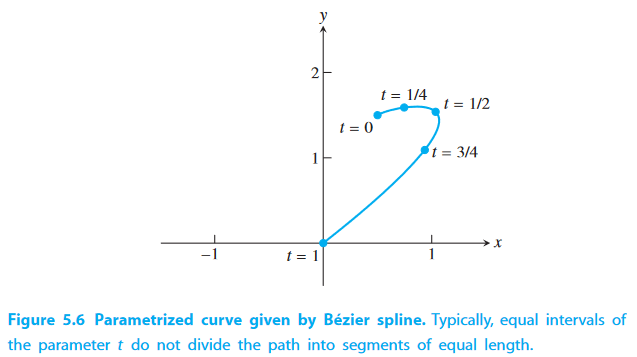
\includegraphics[width=8cm]{myndir/skmyndbok.png}
\centering
\caption{Skýringarmynd úr bók}
\label{skmynd}
\end{figure}


\section{Liður}%liður 1
\subsection{Verkefnalýsing}
Í fyrsta lið á að skrifa kóða fyrir fallið f($\theta$) sem hefur breyturnar $L_1,L_2,L_3\gamma,x_1,x_2,y_2$ sem eru allt fastar og lengd festistanga sem táknaðar eru með $p_1,p_2,p_3$, sem verða þekktar stærðir fyir stöðu kerfis.

\subsection{lausn}


\section{Liður}%liður 2
\subsection{Verkefnalýsing}
Teiknið $f(\theta)$ á bilinu $[-\pi , \pi]$
\subsection{lausn}


\section{Liður}%liður 3
\subsection{Verkefnalýsing}
Teiknið mynd 2 í matlab, báðar stöður samsvara $p_1=p_2=p_3=\sqrt{5}$ og þríhyrningurinn er fenginn með $L_1=L_2=L_3=\sqrt{2},\gamma=\dfrac{\pi}{2}$

\begin{figure}[ht!]
\includegraphics[width=8cm]{myndir/endurteiknimynd.png}
\centering
\caption{mynd til endurteikningar úr bók}
\label{hermi mynd}
\end{figure}

\subsection{lausn}


\section{Liður}%liður 4
\subsection{Verkefnalýsing}%Solve the forward kinematics problem for the planar Stewart platform specified by √x1 =5,(x2,y2)=(0,6),L1 =L3 =3,L2 =3 2,γ =π/4,p1 =p2 =5,p3 =3.Beginby plotting f (θ ). Use an equation solver to find all four poses, and plot them. Check your answers by verifying that p1,p2,p3 are the lengths of the struts in your plot.
Leysið forward kinematics problem fyrir tvívíðan Stewart platorm með gildin
\begin{equation*}
    x_1 =5,(x_2,y_2)=(0,6), L_1 = L_3 =3, L_2 =3\sqrt{2}, \gamma =\dfrac{\pi}{4}, p_1=p_2=5, p_3=3
\end{equation*}
Teiknið $f(\theta)$ og leysið jöfnurnar til að finna allar 4 mögulegar stöður kerfisins og teiknið þær, staðfestuð svörin með að sýna að $p_1,p_2,p_3$ á teikningum séu þau sömu og gefin gildi
\subsection{lausn}


\section{Liður}%liður 5
\subsection{Verkefnalýsing}%Change strut length to p2 = 7 and re-solve the problem. For these parameters, there are six poses.
Breytið undirstöðulengd $p_2=7$ og leystu aftur, fyrir þessi gildi eru 6 mögulegar stöður kerfisins

\subsection{lausn}


\section{Liður}%liður 6
\subsection{Verkefnalýsing}%6. Find a strut length p2, with the rest of the parameters as in Step 4, for which there are only two poses.
Finnið lengd fyrir $p_2$, þar sem stærðir eru annars þær sömu og í lið 4, sem hefur einungis tvær stöður mögulegar
\subsection{lausn}


\section{Liður}%liður 7
\subsection{Verkefnalýsing}
Reiknið bilin fyrir $p_2$, þar sem stærðir eru annars þær sömu og í lið 4, sem hafa 0,2,4 og 6 stöður
\subsection{lausn}



\end{document}
